\documentclass[]{LASPreport}

\usepackage[usenames,dvipsnames]{xcolor}
\usepackage{hyperref}

\newcommand{\SubSystem}{ADCS}
\newcommand{\SERnumber}{ADCS Coarse Sun Sensor Sun Point Estimation Unit Test}
\newcommand{\AgileRevisionNumber}{N/A}
\newcommand{\subject}{Unit Test Results for CSS Sun Point Estimation}
\newcommand{\status}{Initial Test Results}
\newcommand{\preparer}{S. Piggott}
\newcommand{\summary}{
   This is a report documenting the results of the unit test performed for the 
   coarse sun sensor sun point vector estimmation algorithm.}


\begin{document}


\makeCover


%
%	enter the revision documentation here
%	to add more lines, copy the table entry and the \hline, and paste after the current entry.
%
\pagestyle{empty}
{\renewcommand{\arraystretch}{2}
\noindent
\begin{longtable}{|p{0.5in}|p{4.5in}|p{1.14in}|}
\hline
{\bfseries Rev}: & {\bfseries Change Description} & {\bfseries By} \\
\hline
Draft & Initial Revision & S. Piggott \\
\hline

\end{longtable}
}

\newpage
\setcounter{page}{1}
\pagestyle{fancy}

\tableofcontents
~\\ \hrule ~\\

\section{Introduction}
When in safe mode, the spacecraft uses its coarse sun sensors in order to 
point the vehicle's solar arrays at the Sun.  This is done in order to ensure 
that the vehicle gets to a power-positive state with a minimum set of sensors 
in order to recover from whatever event triggered the transition to safe mode.  
The vehicle notionally has 8 coarse sun sensor (CSS) sensors available to it 
which allows it to resolve the exact sun direction in almost all body axes as 
long as all sensors are functional. 

Since there are so many CSSs available, the algorithm needs to be able to obtain 
the sun pointing vector that best fits the current outputs from all of the CSSs.  
This is done by a least squares estimation process that provides the sun vector 
that best fits from a weighted least squares perspective.  The weights are 
simply set based on the current output of each sensor which ensures that the 
sensors that have the best measurements are trusted the most.  The details of 
this algorithm are available in Steve O'Keefe's PhD dissertation. 
\footnote{\href{http://gradworks.umi.com/3704787.pdf}
   {O'Keefe Public Dissertation Link}}

The algorithm stores its internal variables in the CSSWLSConfig data structure 
with the input message coming from the "css\_data\_aggregate" message and the 
output sun pointing vector going to the "css\_wls\_est" message.  This 
algorithm does not use any information stored from previous frames so it is a 
fresh computation every time it is called.  It can therefore be called at any 
rate needed by the system.

\section{Test Design}
The unit test for the cssWlsEst module is located in:\\

\noindent
{\tt FswAlgorithms/attDetermination/CSSEst/UnitTest/CSSWlsEstUnitTest.py} \\
\\

Please see the python script for information on test setup and initial 
conditions.  \\

\noindent This unit test is designed to functionally test the algorithm 
outputs as well as get complete code path coverage.  The test design is broken 
up into four main parts:\\
\begin{enumerate}
\item{Main Body Axis Estimates: The principal body axes (b1, b2, b3) are tested 
   with both positive and negative values to ensure that all axes are correctly 
   estimated.}
\item{Double Coverage Test: There are small regions of pointing where only two 
   sun sensors provide "good" values, which results in a case where only the 
   minimum norm solution can be used instead of a full least squares solution.  
   One of these regions is tested here.}
\item{Single Coverage Test: One of the sensors used for the double coverage test 
   is zeroed in order to simulate a sensor failure and hit the single coverage 
   code.  The accuracy of this estimate is severely compromised.}
\item{Zero Coverage Case: The case where no sensors provide an above-threshold 
   value is tested here.}
\end{enumerate}


\section{Test Results}

The values obtained in the test over time are best visualized in 
Figure~\ref{fig:point_fig}.  That shows a comparison between the Sun pointing 
vector input to the test and the estimate provided by the algorithm.
\begin{figure}[htb]
        \centerline{
        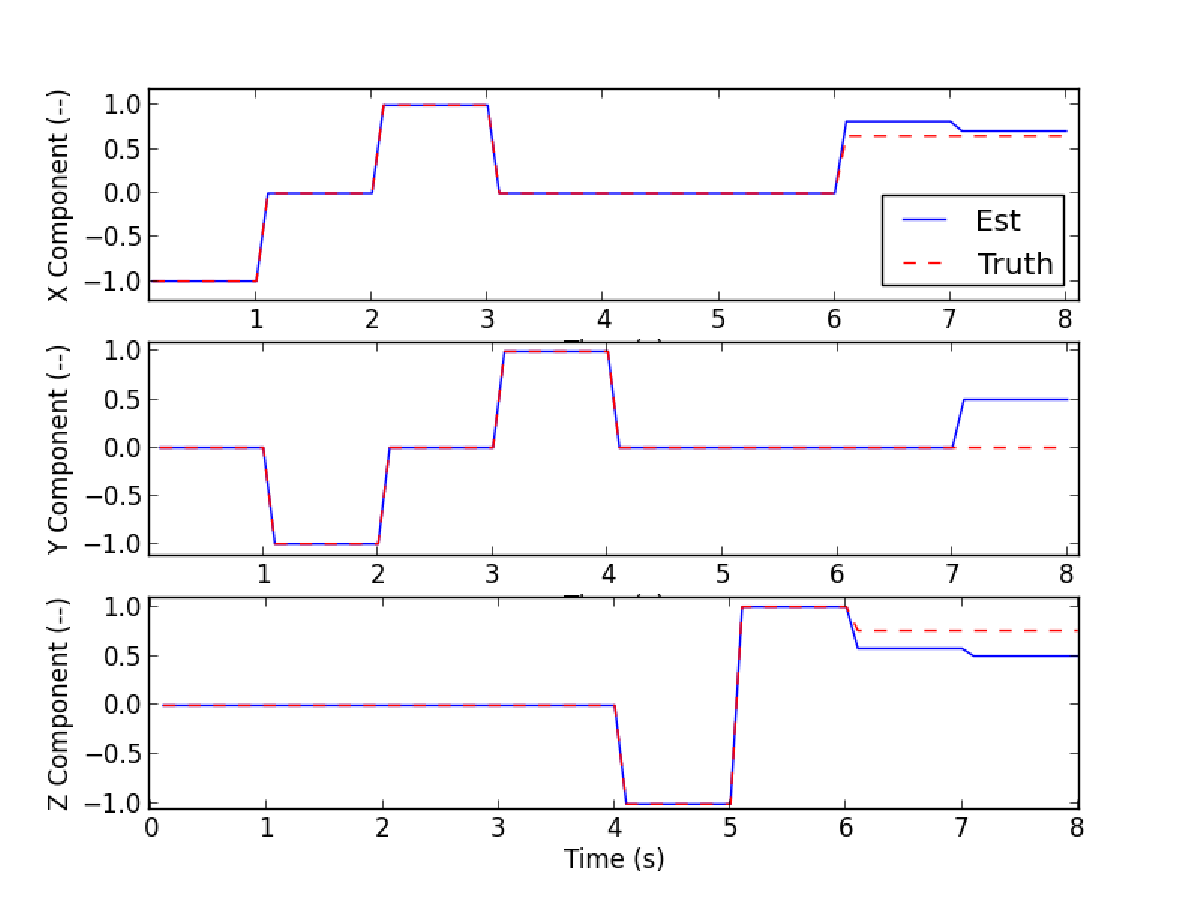
\includegraphics[scale=0.5]{Figures/sunEstAccuracy}
        }
        \caption{Truth and Estimated Sun Pointing Vector}
        \label{fig:point_fig}
\end{figure}

As this plot shows, the algorithm is very accurate up until we hit 6.0 seconds, 
so both directions of the three primary body axes are estimated precisely.  
Then the double coverage case is reasonably accurate, but no longer precise as 
there isn't sufficient information available to get a good pointing direction.  
The single coverage test is not accurate at all (~45 degrees of error), but that 
is simply the best that the algorithm can do with that limited information.

Figure ~\ref{fig:num_fig} shows the number of CSSs used by the algorithm to 
estimate the sun pointing vector over the duration of the test.  It continues 
for longer than Figure~\ref{fig:point_fig} because the algorithm stops setting 
its output message once it gets to the zero valid sensors case as there is no 
good information to provide.
\begin{figure}[htb]
        \centerline{
        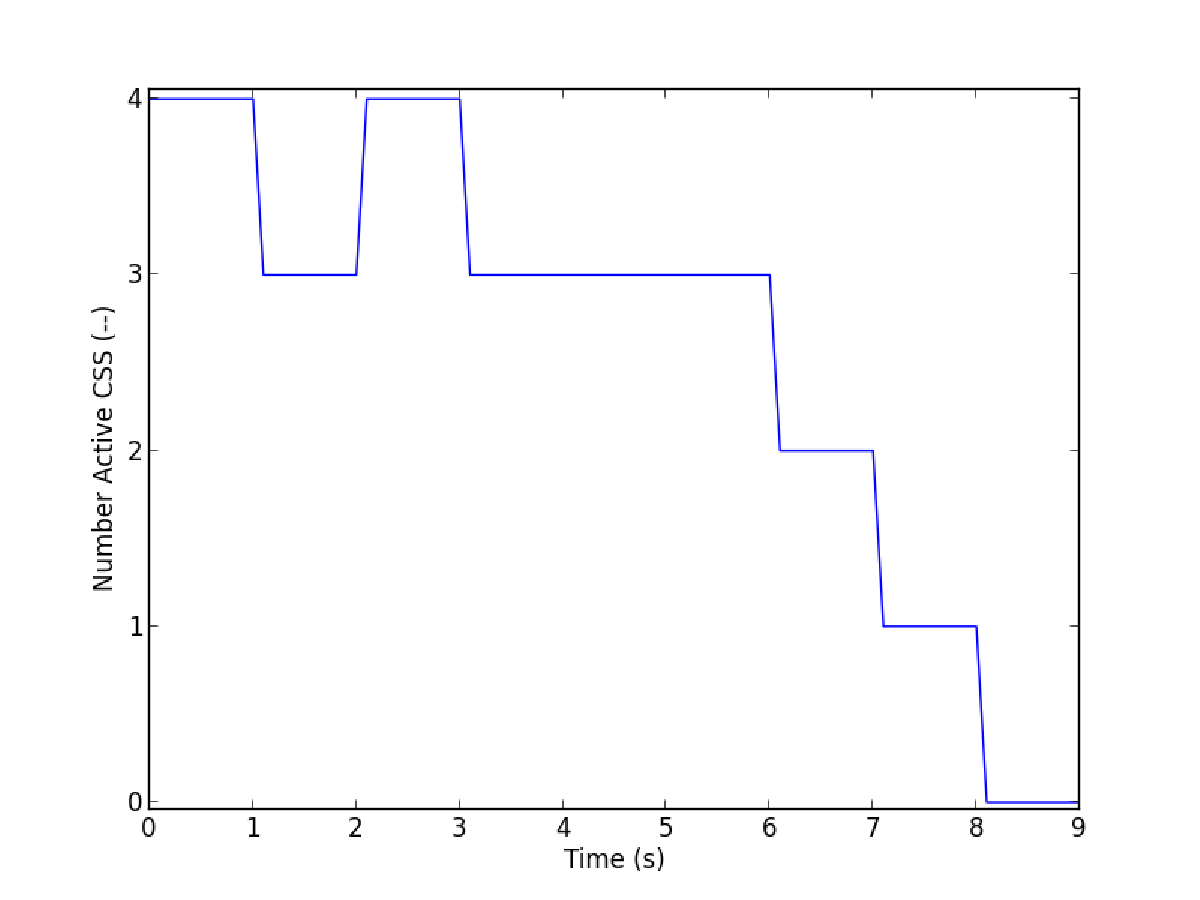
\includegraphics[scale=0.5]{Figures/numGoodCSS}
        }
        \caption{Number of CSSs Used in Estimate}
        \label{fig:num_fig}
\end{figure}


\begin{enumerate}
\item{Main Body Axis Estimates: The sun pointing estimation algorithm is not 
   required to provide a precise estimate of the Sun direction.  This algorithm 
   is only intended to be used in safe mode where the arrays only need to be 
   approximately pointed at the Sun.  For this reason, a pointing vector 
   was flagged as successful when it provided the Sun direction within 17.5 
   degrees which corresponds to a cosine loss of approximately 5\%.  All body 
   axes met this criteria with large margins.  A check was also performed that 
   verified that the predicted number of CSSs matched up with what the 
   algorithm used and this check was also 100\% successful.  The UseWeights flag 
   was initially set to False, and then was changed to True after two cases to 
   ensure that the algorithm works correctly in both cases. 
    \textcolor{ForestGreen}{Test successful.}}
\item{Double Coverage Test: The same accuracy criteria was used for this test.  
   This is mostly a function of CSS geometry and it is also the main driving 
   case for the success criteria used.  It was correct to within 14 degrees. 
   The predicted number of CSSs used (2) also matched the algorithm's selection. 
    \textcolor{ForestGreen}{Test successful.}}
\item{Single Coverage Test: The single coverage case did not have its accuracy 
   tested as there are no accuracy requirements for this case.  It simply must 
   provide an estimate and exit.  The predicted number of CSSs used (1) did  
   match the algorithm's selection.  \textcolor{ForestGreen}{Test successful.}}
\item{Zero Coverage Test: The zero coverage test is only provided here to 
   demonstrate that the algorithm passivates its outputs without hitting any 
   unacceptable event.  It does correctly flag that no valid CSSs were found 
   during the test. \textcolor{ForestGreen}{Test successful.}}
\end{enumerate}

\section{Test Coverage}
The method coverage for all of the methods included in the cssWlsEst 
module are tabulated in Table~\ref{tab:cov_met}

\begin{table}[htbp]
    \caption{ADCS Coarse Sun Sensor Estimation Coverage Results}
   \label{tab:cov_met}
        \centering \fontsize{10}{10}\selectfont
   \begin{tabular}{c | r | r | r} % Column formatting, 
      \hline
      Method Name    & Unit Test Coverage (\%) & Runtime Self (\%) & Runtime Children (\%) \\
      \hline
      SelfInit\_cssWlsEst& 100.0 & 0.0 & 0.0 \\
      CrossInit\_cssWlsEst & 100.0 & 0.0 & 0.0 \\
      computeWlsmn & 100.0 & 0.01 & 0.64 \\
      Update\_cssWlsEst & 100.0 & 0.04 & 0.88 \\
      \hline
   \end{tabular}
\end{table}

For all of the code this test was designed for, the coverage percentage is 
100\%.  For Safe Mode, we do expect this algorithm to be the highest usage 
element from an ADCS perspective, so the CPU usage is almost certainly fine as 
is.  The main penalty comes from the use of matrix multiply in the computeWlsmn 
function.  The only issue of note here is that the matrix multiply algorithm(s) 
use in the FSW should be optimized as much as possible as they are major sources 
of CPU spin.

\section{Conclusions}
The safe mode sun vector estimator described in this document is functionally 
ready from a PDR perspective.  It has no noted failure cases, all code is tested 
for statement coverage, and it successfully meets its test criteria for all 
cases.  The only area where there might be a question is the desired behavior 
for zero-coverage cases.  We may wish to change the outputs to something more 
obviously in-error instead of just having the algorithm go silent.

\end{document}
